\chapter{Эксперименты, ограничения, обсуждение} \label{chaptEval}

В рамках экспериментального исследования и апробации проводилось, в основном, изучение предложенного в данной работе алгоритма синтаксического анализа, архитектуры реализованного инструментария и предложенного метода, так как это является основными результатами данной работы. Так как многие свойства алгоритма либо формально доказаны в рамках работы, либо непосредственно следуют из доказанных свойств и описания (например, завершаемость и корректность на определённых классах входных данных), то интерес при экспериментальном исследовании представляет сравнение с аналогичными алгоритмами и оценка производительности.


\section{Экспериментальная оценка алгоритма}\label{SyntTestsEvalDescr}

Алгоритм синтаксического анализа динамически формируемых выражений, описанный выше, был протестирован на нескольких сериях синтетических тестов, цель которых~--- убедиться в приемлемой производительности алгоритма на практически значимых входных данных. Анализ промышленного проекта по миграции базы данных с MS-SQL Server 2005 на Oraclе 11gR2 показал, что запросы часто формируются конкатенацией фрагментов, каждый из которых формируется с помощью ветвлений или циклов. Ниже приведена эталонная грамматика $G_t$, использованная в этих тестах.

$$
\begin{array}{crcl}
& start\_rule &::=& s \\
& s & ::= & s \mbox{\texttt{ PLUS }} \mbox{\texttt{n}}\\
& n & ::= & \mbox{\texttt{ONE | }} \mbox{\texttt{TWO | }} \mbox{\texttt{THREE | }} \mbox{\texttt{FOUR | }} \\
&   &     & \mbox{\texttt{FIVE | }} \mbox{\texttt{SIX | }} \mbox{\texttt{SEVEN}}
\end{array}
$$

Входные данные представляли собой конечные автоматы над алфавитом терминальных символов грамматики $G_t$, построенные с помощью конкатенации базовых блоков. Предполагается, что такие графы могут быть получены в результате построения регулярной аппроксимации по некоторой программе и выполнения её лексического анализа. В данном случае базовый блок --- это шаблонный конечный автомат, который используется для построения тестовых конечных автоматов. Каждая серия тестов характеризовалась тремя параметрами: 

\begin{itemize}
  \item $height$~--- количество ветвлений в базовом блоке;
  \item $length$~--- максимальное количество повторений базовых блоков;
  \item $isCycle$~--- наличие в базовом блоке циклов (если ложь, то используются базовые блоки, изображённые на рисунке~\ref{block}, если истина~--- то изображённые на рисунке~\ref{block_loop}).
\end{itemize}

\begin{figure}[h!]
 \centering
 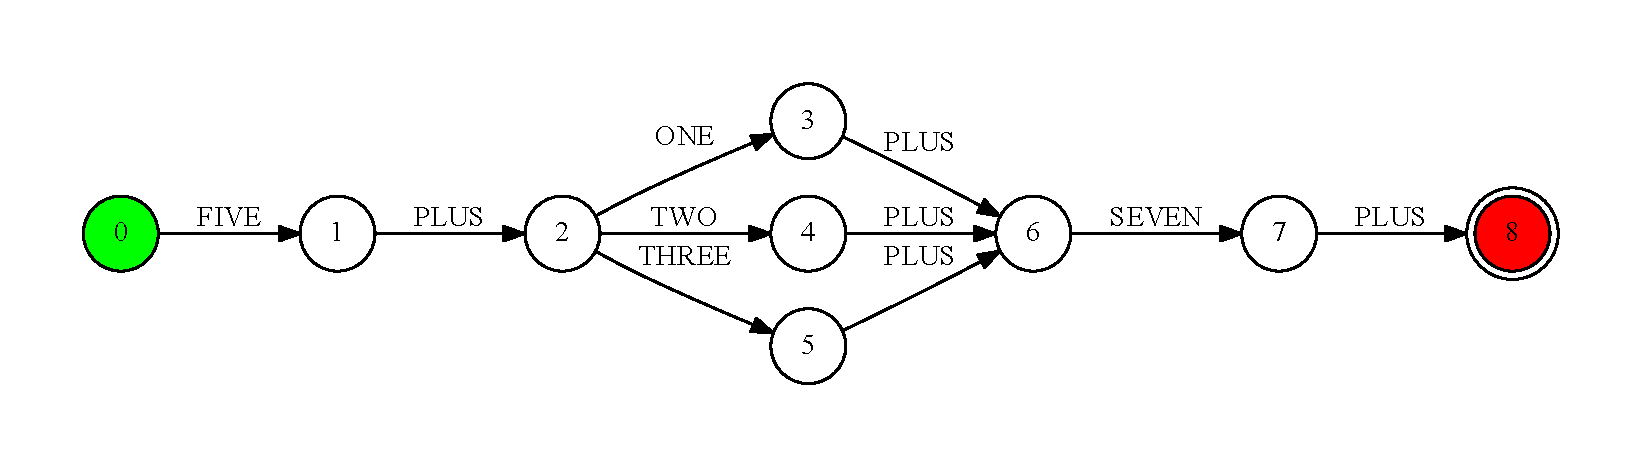
\includegraphics[width=15cm]{pics/block.pdf}
 \caption{Базовый блок без циклов при $height=3$}
 \label{block}
\end{figure}

\begin{figure}[h!]
 \centering
 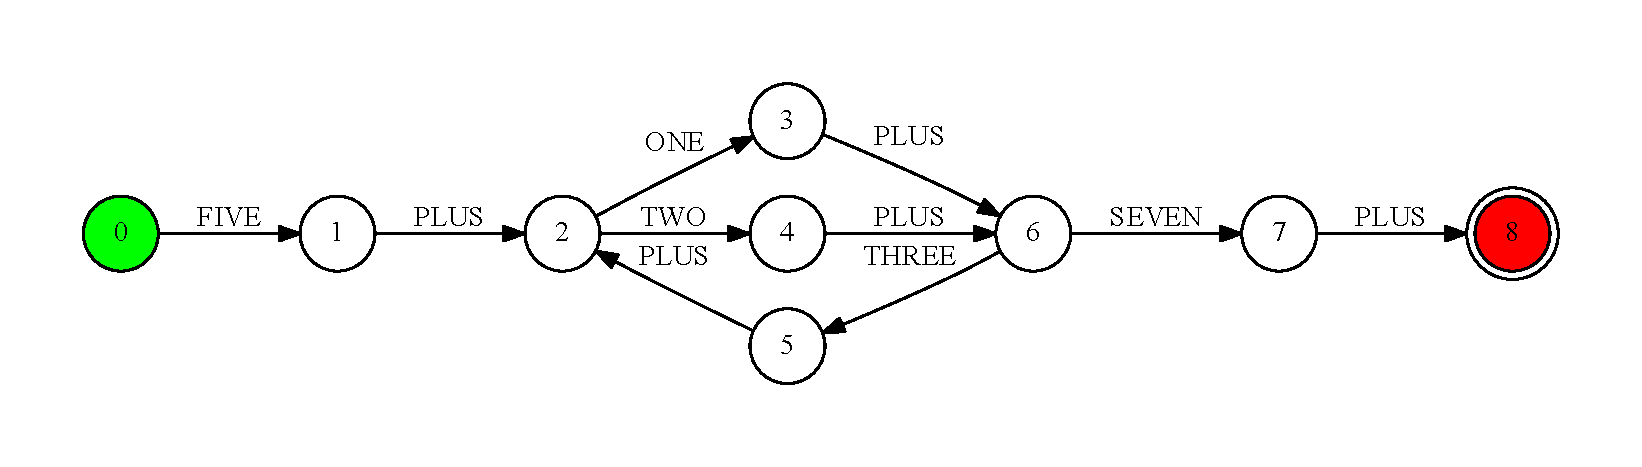
\includegraphics[width=15cm]{pics/block_loop.pdf}
 \caption{Базовый блок, содержащий цикл, при $height=3$}
 \label{block_loop}
\end{figure}

Замеры проводились на вычислительной станции со следующими характеристиками.
\begin{itemize}
\item Операционная система: Microsoft Windows 8.1 Pro
\item Тип системы: x64-based PC
\item Процессор: Intel(R) Core(TM) i7-4790 CPU @ 3.60GHz, 3601 Mhz, 4 Core(s), 8 Logical Processor(s)
\item Объём оперативной памяти: 16.0 GB
\end{itemize}

Чтобы выявить зависимость времени от размера входных данных, тесты проводились сериями. Каждая серия объединяет набор из $500$ тестов, каждый из которых содержит одинаковое количество ветвлений в базовом блоке. При этом количество повторений блока совпадает с порядковым номером теста, то есть $length=i$ для $i$-того теста. Для каждого теста измерялось время, затраченное на синтаксический анализ. Измерения проводились 10 раз, после чего усреднялись. График, представленный на рисунке~\ref{diffheights}, иллюстрирует зависимость времени, затрачиваемого на синтаксический анализ, от количества повторения базового блока и количества ветвлений в каждом из них. Можно заметить, что время, затрачиваемое на анализ, растёт линейно, в зависимости от размера входного графа. График на рисунке~\ref{CycleVsLinear} показывает, что наличие циклов в графе, при одинаковом значении параметра $height$, увеличивает продолжительность анализа, при этом зависимость времени от размера графа остаётся линейной.

\begin{figure}[h!]
 \centering
 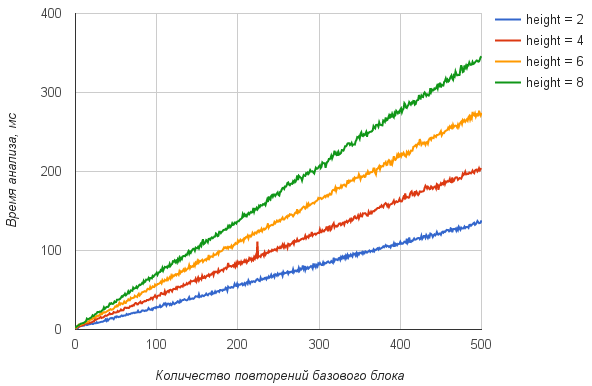
\includegraphics[width=15cm]{pics/diffheights.png}
 \caption{Зависимость времени работы алгоритма от размера входного графа при $isCycle=false$}
 \label{diffheights}
\end{figure}

\begin{figure}[h!]
 \centering
 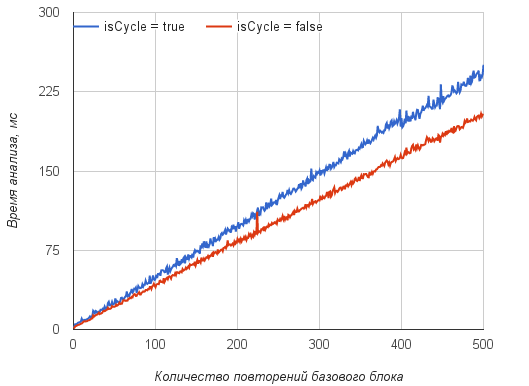
\includegraphics[width=15cm]{pics/heigh4.png}
 \caption{Зависимость времени работы алгоритма от размера входного графа и наличия в нем циклов при $height=4$}
 \label{CycleVsLinear}
\end{figure}


\section{Сравнение с инструментом Alvor}

Отдельно было приведено сравнение производительности синтаксического анализа с инструментом Alvor, так как он реализует очень близкий подход: независимые шаги анализа, синтаксический анализ основан на GLR-алгоритме.

Так как Alvor не предоставляет платформы для простой реализации поддержки новых языков, то для сравнения было выбрано подмножество языка SQL, общее для Alvor и реализованного в рамках апробации инструмента. Тесты строились по принципу, аналогичному изложенному в разделе~\ref{SyntTestsEvalDescr}.

!!!Далее сколько-то картинок и выводы!!!


\section{Апробация в промышленном проекте по реинжинирингу}

Реализованный инструментарий был апробирован в рамках промышленного проекта по миграции базы данных с MS-SQL Server 2005 на Oraclе 11gR2, что позволило апробировать как предложенную методику, так и протестировать некоторые части инструментария на реальных данных.

Обрабатываемая система состояла из 850 хранимых процедур и содержала около 2,6 миллионов строк кода. В ней присутствовало 2430 точек выполнения динамических запросов, из которых больше 75\% могли принимать более одного значения и при их формировании использовалось от 7 до 212 операторов. При этом среднее количество операторов для формирования запроса равнялось 40.

Ранее в данном проекте использовался алгоритм, предложенный и реализованный автором данной работы, детали которого описаны в статье~\ref{!!!}. Поэтому требовалось внедрить новый алгоритм синтаксического анализа в уже существующую инфраструктуру. Однако так как вопрос выполнения трансляции над SPPF не исследован и его изучение не входило в данную работу, а возможность извлечения конечного числа деревьев, что аналогично ранее используемому алгоритму, была показана ранее, то в в рамках данной апробации ставилась иная задача. Было необходимо вычислить набор метрик динамически формируемого кода непосредственно по SPPF. 

Для вычисления были выбраны, на основе работ~\cite{DSQLQualityMesure, DSQLQualityMesureBIG, DevelopmentDSQLTools}, следующие метрики.
\begin{itemize}
    \item Количество используемых в запросе таблиц.
    \item    
    \item 
\end{itemize}

Действия по созданию инструмента подтвердили изложенную ранее методику. Так как анализатор T-SQL был разработан ранее, то была взята готовая грамматика и по ней построен синтаксический анализатор. Построение регулярной аппроксимации и лексический анализ были переиспользованы, что показало преимущества разделения шагов анализа.

Далее были реализованы функции вычисления метрик и вывода результата, после чего полученная функциональность была встроена в существующую цепочку обработки основного кода.

В результате работы реализованных функций формировался отчёт, пример которого приведён в таблице~\ref{tbl:metrics}

\begin{table} [htbp]
  \centering
  \parbox{14cm}{\caption{Пример метрик}\label{tbl:metrics}}
  \begin{tabular}{| p{2.6cm} || p{2cm} | p{1.8cm} | p{1.8cm} | p{1.8cm} | p{2cm} | p{2cm}l |}
  \hline                               
  \hline
  \small{Инструмент}   &\centering \small{Платформа} &\centering \small{Лес разбора}      &\centering \small{Синт. ошибки} &\centering \small{Сем. ошибки} &\centering \small{Подсветка} &\centering \small{Модульность} & \\
  \hline 
  AbsPars      &\centering  $-$      &\centering  $+-^1$                 &\centering  $+$                  &\centering  $+$                 &\centering  $-$                 &\centering  $-$        & \\
  Alvor        &\centering  $-$      &\centering  $-$                    &\centering  $+$                  &\centering  $-$                 &\centering  $-$                 &\centering  $+$        &\\
  JSA          &\centering  $-$      &\centering  $-$                    &\centering  $+$                  &\centering  $-$                 &\centering  $-$                 &\centering  $-$        &\\
  PHPSA        &\centering  $-$      &\centering  $-$                    &\centering  $+$                  &\centering  $-$                 &\centering  $-$                 &\centering  $-$        &\\
  IntelliLang  &\centering  $+-^3$   &\centering  $-$                    &\centering  $+$                  &\centering  $+$                 &\centering  $+$                 &\centering  $+$        &\\
  Varis        &\centering  $-$      &\centering  $+^2$                  &\centering  $+$                  &\centering  $-$                 &\centering  $+$                 &\centering  $-$        &\\
  YC           &\centering  $+$      &\centering  $+$                    &\centering  $-^4$                &\centering  $+$                 &\centering  $+$                 &\centering  $+$        &\\
  \hline
  \hline
  \end{tabular}
\end{table}

Возможно, какое-то обсуждение + сравнение с аналогичными результатами на старом движке.

Алгоритм синтаксического анализа был отдельно протестирован на наборе данных, взятых из описанного выше проекта. Реализация алгоритма была внедрена в проект по миграции, заменив ранее используемую версию алгоритма синтаксического анализа. При этом грамматика языка T-SQL была полностью переиспользована. Алгоритм запускался на данной системе 10 раз, время анализа усреднялось. Тесты проводились на вычислительном устройстве с параметрами, эквивалентными указанным в разделе~\ref{!!!}

Алгоритм успешно завершил работу на 2188 входных графах, аппроксимирующих множества значений запросов. Ручная проверка входных графов, на которых алгоритм завершался с ошибкой, показала, что они действительно не содержали ни одного корректного в эталонном языке выражения. Причиной этого стала либо некорректная работа лексического анализатора, либо наличие в выражениях конструкций, не поддержанных в существующей грамматике. Дальнейшие значения приводятся только для графов, которые удалось проанализировать. 604 из этих графов содержали ровно один путь и анализировалось не более 1 миллисекунды. Общее время синтаксического анализа составило порядка 27 минут, из них 13 минут было затрачено на разбор графов, не содержащих ни одного корректного выражения. В среднем один такой граф анализировался 386 миллисекунд. На разбор 1790 графов ушло не более 10 миллисекунд. На анализ двух графов было затрачено более 2 минут: 152,215 и 151,793 секунд соответственно. Первый граф содержал 2454 вершин и 54335 рёбер, второй~--- 2212 вершин и 106020 рёбер. Распределение входных графов по промежуткам времени, затраченных на анализ, приведено на графике на рисунке~\ref{distr}.

\begin{figure}[H]
  \centering
 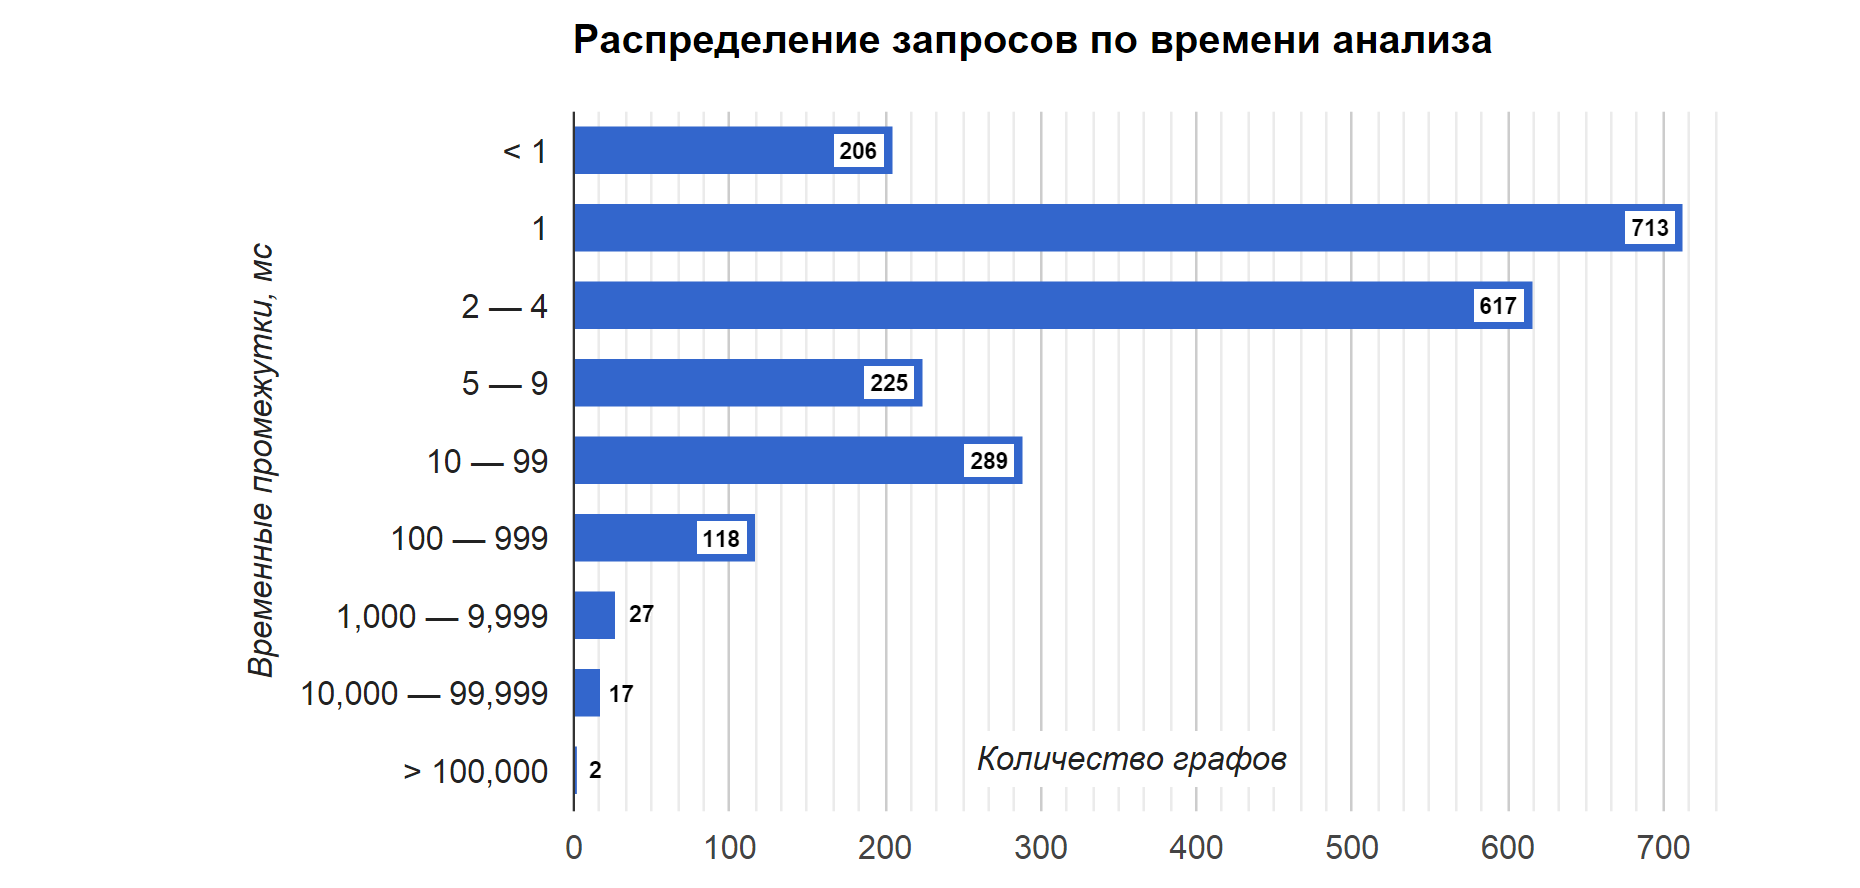
\includegraphics[width=0.95\textwidth]{pics/distr.png}
 \caption{Распределение запросов по времени анализа}
 \label{distr}
\end{figure}

Результаты данных замеров показывают, что ресурсоёмкость синтаксического анализа уменьшилась, так как при использовании нового алгоритма только один запрос не был обработан из-за превышения времени, отведённого на вычисления. В предыдущей версии количество таких запросов равнялось !!!!~\cite{Syrcose}. Это позволяет повысить уровень автоматизации, так как большее количество запросов можно обработать автоматически.

Тестирование на реальных данных показало, что предложенный в работе алгоритм синтаксического анализа применим для синтаксического анализа регулярной аппроксимации множества значений динамически формируемых выражений, используемых в коде промышленных информационных систем. Также данная апробация показала, что предложенная методика применима при разработке средств реинжиниринга, а модульность позволяет использовать отдельные инструменты независимо. В ходе апробации были выявлены особенности, на которые следует обратить внимание при исследовании вопроса о вычислении семантики непосредственно над SPPF. Результаты успешно внедрены в проект компании ЗАО ``Ланит-Терком''.


\section{Разработка расширений для поддержки встроенных языков}

На основе YC.SEL.SDK и YC.SEL.SDK.ReSharper, которые были представлены ранее, в рамках апробации были реализованы расширения к ReSharper, которые предоставляют поддержку для  двух встроенных языков языков: подмножества T-SQL и Calc. Реализация данных расширений также являлась апробацией предложенной методики использования разработанного инструментального пакета.

В рамках предложенной методики были созданы лексические спецификации и грамматики соответствующих языков. Исходный код описаний опубликован в открытом доступе: \url{https://github.com/YaccConstructor/YC.GrammarZOO}. Далее с помощью генераторов из разработанного инструментария, по этим грамматикам построены синтаксические анализаторы, а по лексическим спецификациям --- лексические анализаторы.

При создании расширений был также апробирован механизм построения регулярной аппроксимации. Для построения графа потока управления внешнего вода использовалась функциональность ReSharper SDK. Затем полученный граф переводился в обобщённое представление, по которому строилась регулярная аппроксимация силами разработанного инструмента.

После того, как отдельные части были готовы, они собирались в единое целое на основе YC.SEL.SDK.ReSharper. В результате было получено два расширения, предоставляющие поддержку соответствующих языков и ядро, содержащее общую, независимую от языков, функциональность, связанную прежде всего с обеспечением взаимодействия между ReSharper и реализованными расширениями.

Расширения предоставляют следующую функциональность: подсветка синтаксиса (рисунок~\ref{fig:sHiglighting}), подсветка парных (рисунок~\ref{fig:braces}) элементов. Для языка Calc также реализована статическая диагностика семантических ошибок, а именно поиск использования необъявленных переменных, что показывает, с одной стороны, возможность непосредственного использования SPPF для проведения анализа динамически формируемого кода, а с другой --- возможность реализации дополнительной функциональности, не являющейся общей функциональностью SDK.

Статический поиск использования необъявленных переменных показан на 
рисунке~\ref{fig:undeclaredVars}. В данном примере переменная \verb|x| объявляется в одной из веток условного оператора и не объявляется в другой, что может привести к ошибке в точке использования, о чём и сообщено пользователю.

\begin{figure}[H]
  \centering
 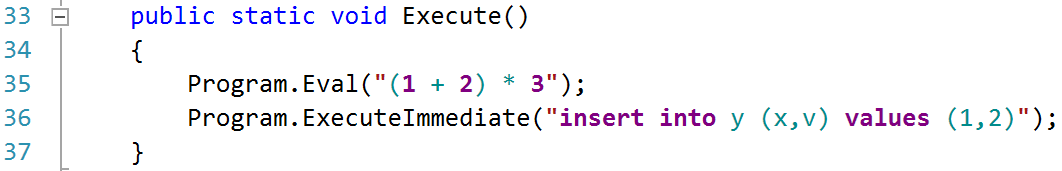
\includegraphics[width=0.95\textwidth]{pics/multilanguages_light.png}
 \caption{Пример подсветки синтаксиса для нескольких встроенных языков: SQL и Calc}
 \label{fig:sHiglighting}
\end{figure}

\begin{figure}[H]
 \centering
 \begin{subfigure}[b]{0.47\textwidth}
  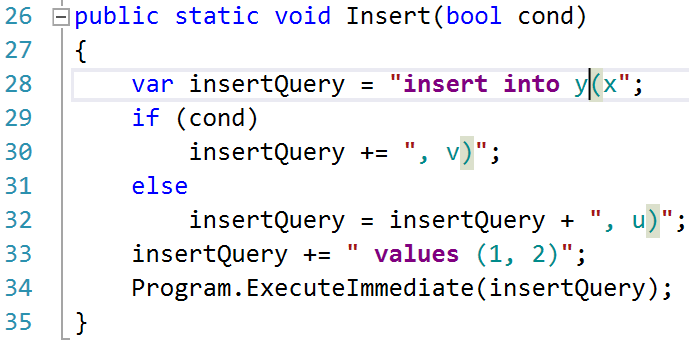
\includegraphics[width=\textwidth]{pics/brackets_one_to_many_light.png}
  \caption{Одной открывающей скобке соответствует несколько закрывающих}
  \label{fig:brOneToMany}
  \end{subfigure}
  ~
 \begin{subfigure}[b]{0.47\textwidth}
  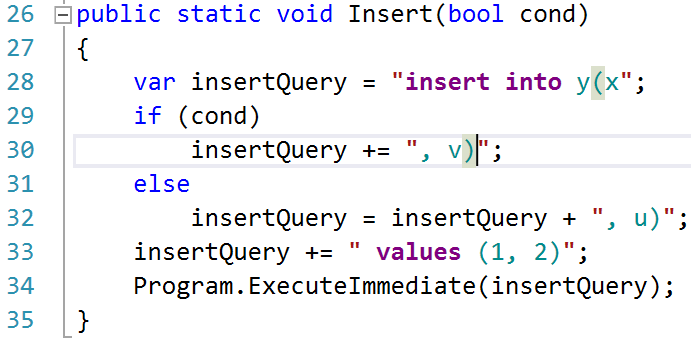
\includegraphics[width=\textwidth]{pics/brackets_one_to_one.png}
  \caption{Одной закрывающей скобке соответствует одна открывающая}
  \label{fig:brOneToone}
 \end{subfigure}

 \caption{Пример подсветки парных скобок}
 \label{fig:braces}
\end{figure}

\begin{figure}[H]
  \centering
 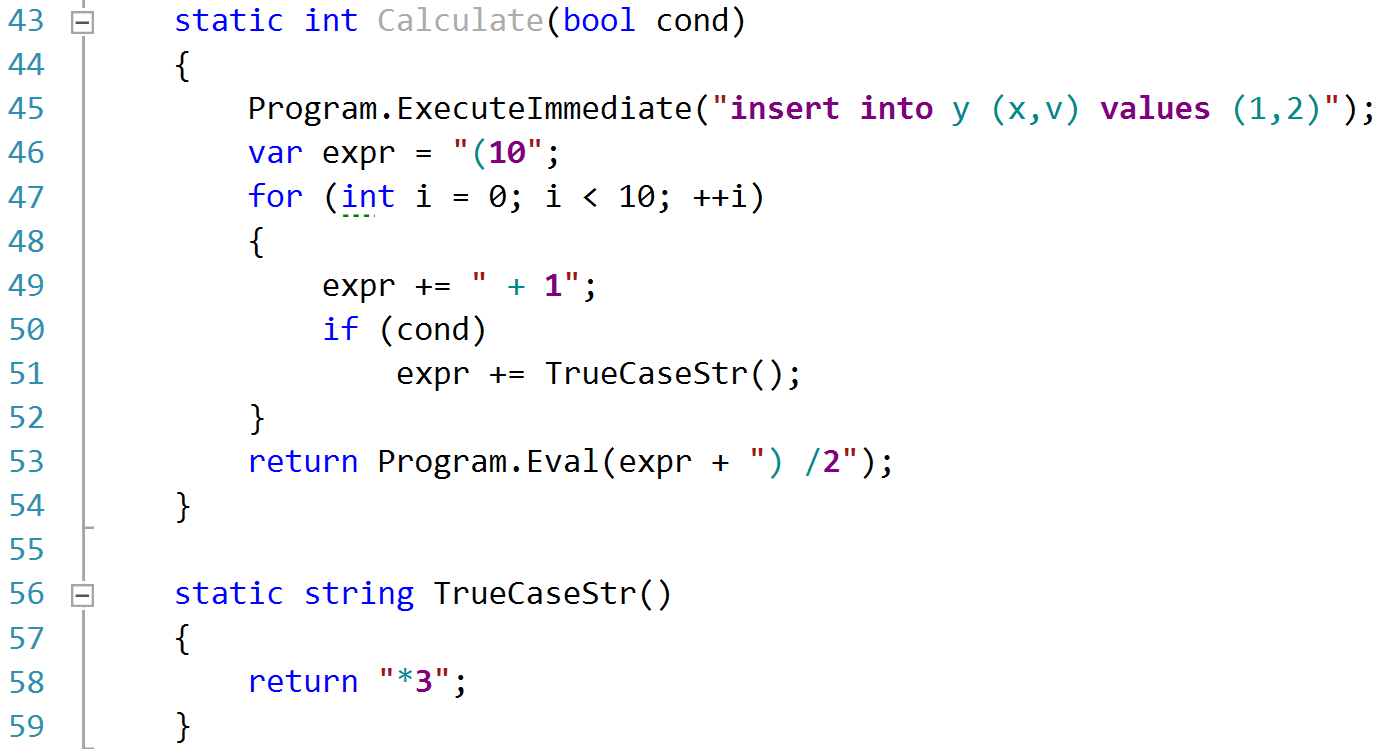
\includegraphics[width=0.95\textwidth]{pics/sql_calc_cycle.png}
 \caption{Пример межпроцедурной обработки встроенных языков}
 \label{fig:interProc}
\end{figure}

\begin{figure}[H]
  \centering
 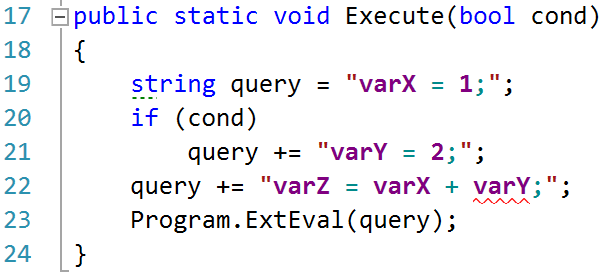
\includegraphics[width=0.75\textwidth]{pics/undefined_variable.png}
 \caption{Пример статического обнаружения семантических ошибок для языка Calc}
 \label{fig:undeclaredVars}
\end{figure}

Расширения опубликованы в виде готовых к использованию бинарных пакетов. Функциональность, отвечающая за поддержку каждого языка, распространяется в виде самостоятельного бинарного пакета и может быть независимо подключена или отключена. Структура пакетов представлена на рисунке~\ref{fig:packagesStructure}.

\begin{figure}[H]
  \centering
 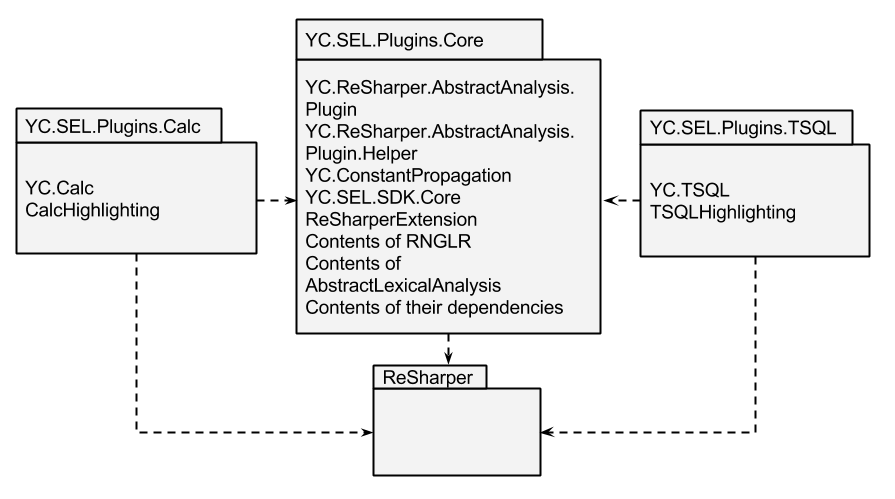
\includegraphics[width=0.90\textwidth]{pics/RshPluginsPackages.png}
 \caption{Структура пакетов расширений для ReSharper, предоставляющих поддержку встроенных T-SQL и Calc}
 \label{fig:packagesStructure}
\end{figure}

Дополнительно в результате разработки расширений было выяснено, что анализаторы языков могут быть независимо переиспользованы. Например, они используются в тестах, никак не связанных с ReSharper. Это показывает, что независимость шагов обработки динамически формируемых выражений позволяет достаточно просто переиспользовать компоненты, реализующие эти шаги, что является плюсом реализованного решения.

\section{Ограничения}

Используемые подходы и алгоритмы накладывают ограничения на платформу и разрабатываемые на её основе инструменты. Обсуждению этих ограничений посвящён данный раздел.

Множество, являющееся аппроксимацией множества значений динамически формируемого выражения, принимаемое на вход алгоритмом синтаксического анализа должно быть регулярным множеством. То есть аппроксимация задаёт регулярный язык, в то время как генерируемый программой может быть регкурсивно-перечислимым. Это означает, что за на этапе построения аппроксимации будет происходить потеря точности. Например, нехвостовая рекурсия точно не выразима в терминах регулярных множеств. Точность построения конкретной регулярной аппроксимации зависит от конкретного алгоритма, используемого для этого. алгоритм может реализовывать или не реализовывать межпроцедурный анализ, поддерживать или не поддерживать строковые операции, разными способами обрабатывать пользовательский ввод и другие ситуации, когда значение выражения вычислить невозможно. В рамках рассматриваемой платформы реализован алгоритм позволяющий поддерживать межпроцедурный анализ и строковые операции. 

Эталонный язык должен быть описан детерминированной контекстно-свободной грамматикой. Большинство языков программирования могут быть описаны такой грамматикой. Однако, с одной стороны, бывают исключения, например C++. С другой стороны, в документации языка программирования может быть приведена недетеминированная грамматика, а её приведение к детерминированной может потребовать значительных усилий. 

Вопросы быстродействия инструментов, созданных на основе зависят от контекста их использования. Если при реинжиниринге допустимо проведение длительных анализов, то для многих инструментов, используемых  в средах разработки, время отклика критично.  Особенно это важно для функциональности, работающей в режиме ``на лету'': подсветка синтаксиса, автодополениее, подсказки. Так как платформа создавалась с ориентацией на создание инструментов для реинжинирига, то некоторые компоненты направлены на увеличение точности анализа, возможно, в ущерб производительности. Примером такой компоненты может служить компонента построения регулярной аппроксимации, которая реализовывает алгоритм, который гарантирует построение приближения сверху, учитывает циклы и строковые функции~\cite{RegOverApprox}. Это повышает точность анализа, однако производительность может оказаться слишком низкой для использования в IDE. С другой стороны, при создании инструмента для IDE возможно заменить построение аппроксимации на более легковесное, но менее точное. Например в инструменте Alvor~\cite{Alvor2}, предназначенном прежде всего для интерактивной работы в среде разработки, предлагается такой алгоритм.  При этом важно, что возможности платформы позволяют комбинировать различные реализации компонент, так как они независимы. То есть можно использовать один и тот же синтаксический анализатор с разными вариантами лексичекого для получения требуемых характеристик результирующего инструмента. С другой стороны, текущая реализация содержит возможности для различного рода оптимизаций: некоторые алгоритмы могут быть ускорены с помощью распараллеливания, выбор оптимальных структур данных, например для конечных автоматов, активно использующихся в рамках платформы, является темой отдельного исследования~\cite{DataStructureForFA}.

Систематическое исследование работы с SPPF находится на начальной стадии даже в контексте обобщённого синтаксического анализа~\cite{SPPF2015}. В рамках же анализа динамически формируемых выражений исследований в этом направлении не обнаружено. По этой причине в рамках данной работы реализован только прототип библиотеки, позволяющей решать некоторые задачи, например, поиск необъявленных переменных, над SPPF в общем виде. Теоретическое исследование данного вопроса является отдельной задачей. С другой стороны, было доказано, что из построенного SPPF извлекаемы деревья вывода для любых цепочек из аппроксимации, а с деревьями можно работать с помощью стандартных методов. 

\clearpage
